\chapter{Stand van zaken}
\label{ch:stand-van-zaken}

% Tip: Begin elk hoofdstuk met een paragraaf inleiding die beschrijft hoe
% dit hoofdstuk past binnen het geheel van de bachelorproef. Geef in het
% bijzonder aan wat de link is met het vorige en volgende hoofdstuk.

% Pas na deze inleidende paragraaf komt de eerste sectiehoofding.

Dit hoofdstuk is een literatuurstudie over de huidige stand van zaken rond Kotlin. Hierin wordt bekeken wat Kotlin eigenlijk is en waarom Kotlin is uitgevonden. Daarna is Kotlin op verschillende platformen aan de beurt, meer specifieke is dit iOS, Android, webapplicatie en als back-end. Tenslotte het gebruik van Kotlin, hoeveel ontwikkelaars maken er reeds gebruik van Kotlin? Na het lezen van dit hoofdstuk bent u volledig op de hoogte van de laatste nieuwigheden rond Kotlin.

\section{Wat is Kotlin?}
\label{sec:kotlin}
Volgens de FAQ van Kotlin \autocite{JetBrainsFAQ} is Kotlin een open-source programmeertaal die object-georiënteerde en functionele programmatie features combineert. Kotlin is ook een statically typed programmeertaal. Dit betekent dat het type van de variabele is toegekend wanneer de code wordt gecompileerd. Javascript is een dynamically typed programmeertaal, waarbij aan een variabele verschillende types kan worden toegekend. Zo kan een variabele bij Javascript in het begin een getal zijn, maar wat verder in de code kan dit veranderd worden naar een tekst.

Kotlin is ontworpen door JetBrains. JetBrains is een organisatie afkomstig van Sint-Petersburg, Rusland. De naam Kotlin is afkomstig van het Kotlin eiland, 30 km ten westen van Sint-Petersburg. JetBrains is een software ontwikkelingbedrijf dat gesticht is in het jaar 2000. Hun hoofdkantoor is gevestigd in Praag (Tsjechië) en hun core-business is het ontwikkelen van tools die gebruikt kunnen worden door verschillende types van software ontwikkelaars. Zo hebben zij IDE's\footnote{Integrated Development Environment} ontwikkeld voor Java, Ruby, Python, PHP, SQL, Objective-C, C++, C\# en JavaScript \autocite{JetBrainsOverView}.

\section{Kotlin en Android}
\label{sec:kotlinandroid}
Volgens het artikel van \textcite{GoogleSupportKotlin} heeft Google in 2017 bekend gemaakt dat het Kotlin volledig zou ondersteunen voor Android applicatieontwikkeling. In Android Studio zal vanaf versie 3.0 Kotlin ondersteund worden voor Android development. Een Kotlin project maken in Android Studio is dan ook heel gemakkelijk. In Android Studio is er bij het aanmaken van een project de mogelijkheid om direct de ondersteuning voor Kotlin in te schakelen. Hierdoor zal het aangemaakte project onmiddellijk in Kotlin geschreven zijn.

Het is mogelijk in Android Studio om een reeds bestaand Android Java project om te zetten naar Kotlin. Hierbij zal de actie 'Convert Java File to Kotlin File' moeten uitvoerd worden (rechtermuisknop in het Java bestand). Hierdoor zal Android Studio detecteren dat er gebruik gemaakt zal worden van Kotlin, waardoor hij zal vragen om de Kotlin plugin te installeren via Gradle indien deze nog niet is geïnstalleerd.


\section{Automigration}
\label{sec:Automigration}
Door de intergratie van Kotlin in Android Studio werd er een conversietool ter beschikking gesteld. Met behulp van deze tool kan bestaande Java-code eenvoudig worden omgezet naar Kotlin. Dit zorgt ervoor dat veel tijd kan worden bespaard en het programmeren van dubbele code zo wordt vermeden. Maar deze conversietool bevat wel een klein risico. Het kan wel eens gebeuren dat code soms fout wordt geconverteerd. 

Het is ook reeds mogelijk om zowel Java en Kotlin te combineren. Zo kunnen de verschillende object classes in Java worden geschreven en kan je via Kotlin alle objecten aanmaken. Of dit nuttig en best practice is, valt te beslissen door de developer.

Indien bestaande Java code online of van een vorige project gekopieerd en geplakt wordt naar een bestaand Android Studio project, dan zal Android Studio zelf detecteren dat er Java code gebruikt zal worden in een Kotlin project. Hij zal dan zelf ook de suggestie doen om de Java code om te zetten naar Kotlin code \autocite{Avantica2017}.


\section{Kotlin web en back-end}
\label{sec:kotlincrossplatform}
Kotlin kan net zoals Java gebruikt worden om webapplicaties te bouwen. Dit in combinatie met bijvoorbeeld het Spring Framework, waarbij HttpServlets gebruikt worden om de webpagina's te tonen \autocite{JetBrainsWeb}.

Wens je echter een full-stack webapplicatie te bouwen, dan heb je de mogelijkheid om ook een Kotlin server op te zetten. Zo kan je bijvoorbeeld aan de webapplicatie een RESTfull server hangen om verschillende API calls te doen  \autocite{JetBrainsServer}.

Kotlin-applicaties kunnen worden geïmplementeerd op elke host die Java-webapplicaties ondersteunt, inclusief Amazon Web Services, Google Cloud Platform en veel meer. Zowel een Kotlin webapplicatie als back-end maakt gebruik van de JVM.

\section{Kotlin/Native}
\label{sec:kotlinnative}
Waarschijnlijk momenteel één van de meest nieuwe en innovatieve projecten van JetBrains is Kotlin/Native. Momenteel is men gekomen aan versie 0.6 en er zijn al verschillende voorbeeldprojecten beschikbaar gesteld door JetBrains. Kotlin/Native zou het mogelijk maken om éénmalig domeinlogica te schrijven in een applicatie en deze te delen over verschillende platformen, bijvoorbeeld Android en iOS. De user interfaces zou men wel nog per platform moeten opbouwen, waardoor je toch het 'native applicatie'-gevoel krijgt. Kotlin/Native maakt gebruik van een totaal andere compiler dan de Javac (Java) of Kotlinc (Kotlin) compiler die bytecode genereert voor de JVM, zie sectie \ref{sec:llvm} voor meer info. De bijnaam die gegeven wordt aan Kotlin/Native is \textit{Konan}. Binnen dit onderzoek zal Kotlin/Native nauw onderzocht worden \autocite{AlbertGao}.

\section{Verschil tussen Kotlin en Kotlin/Native}
\label{sec:differenceKotlinAndNative}
Het is belangrijk om een duidelijk verschil te zien tussen Kotlin en Kotlin/Native. Met Kotlin spreken we over de programmeertaal. Met Kotlin/Native wordt het framework bedoeld dat gebruikt kan worden voor cross-platform applicatieontwikkeling. Het framework zal gebruik maken van de programmeertaal Kotlin.

\section{Kotlin en iOS}
Verschillende ontwikkelaars, zoals \textcite{GaoIOS}, zijn reeds aan de slag gegaan met deze Kotlin/Native plugin. Op zijn website is te zien hoe het mogelijk is om aan de hand van deze plugin, Kotlin te gebruiken voor iOS development. 

Er zijn twee mogelijkheden. Enerzijds is er de mogelijkheid om het project in Objective-C aan te maken. De code wordt, rechtstreeks in de Objective-C bestanden, in Kotlin geprogrammeerd in combinatie met Objective-C annotations. Anderzijds kan het project in Swift aangemaakt worden. De overige Kotlin code wordt geprogrammeerd in aparte Kotlin bestanden, gecompileerd naar een iOS framework en toegevoegd aan het project.

Alhoewel het niet echt optimaal is om Kotlin direct te programmeren in Xcode, aangezien Xcode een Kotlin bestand niet zal herkennen, is het dus mogelijk. Indien de applicatie enkel en alleen ontwikkeld moet worden voor het iOS platform, dan is en blijft Swift of Objective-C de beste manier om een iOS applicatie te bouwen.

\section{Compiler}
\label{sec:llvm}
Net zoals Java draait Kotlin op de JVM. Dit wil dus zeggen dat alle toestellen die een JVM kunnen draaien, ook Kotlin code ondersteunen. Maar sinds de dag dat JetBrains besloten heeft om zich niet enkel meer te richten op platformen die enkel en alleen de JVM ondersteunen \autocite{JetBrainsVM}, hebben zij ervoor gezorgd dat ongeacht welk platform of besturingssysteem er gebruikt wordt, de Kotlin code wordt ondersteund. Dit komt door de LLVM compiler die Kotlin/Native gebruikt. Deze wordt in hoofdstuk \ref{ch:compiler} verder besproken.

\section{Het gebruik van Kotlin}
\label{sec:kotlingebruik}
Het gebruik van Kotlin is gedurende de jaren zeer sterk gestegen. Op de blog van JetBrains \autocite{JetBrains12} zijn grafieken te vinden waarmee wordt aangetoond dat de populariteit van Kotlin enkel maar stijgt.

Figuur \ref{fig:kotlingithub} toont het aantal lijnen Kotlin code beschikbaar op GitHub, het aantal vragen gesteld op Stackoverflow over Kotlin en het aantal keer dat de Kotlin plugin werd gebruikt. Hieruit kan besloten worden dat het gebruik van Kotlin sterk stijgt de laatste drie jaren.

\begin{figure} [ht]
	\centering
	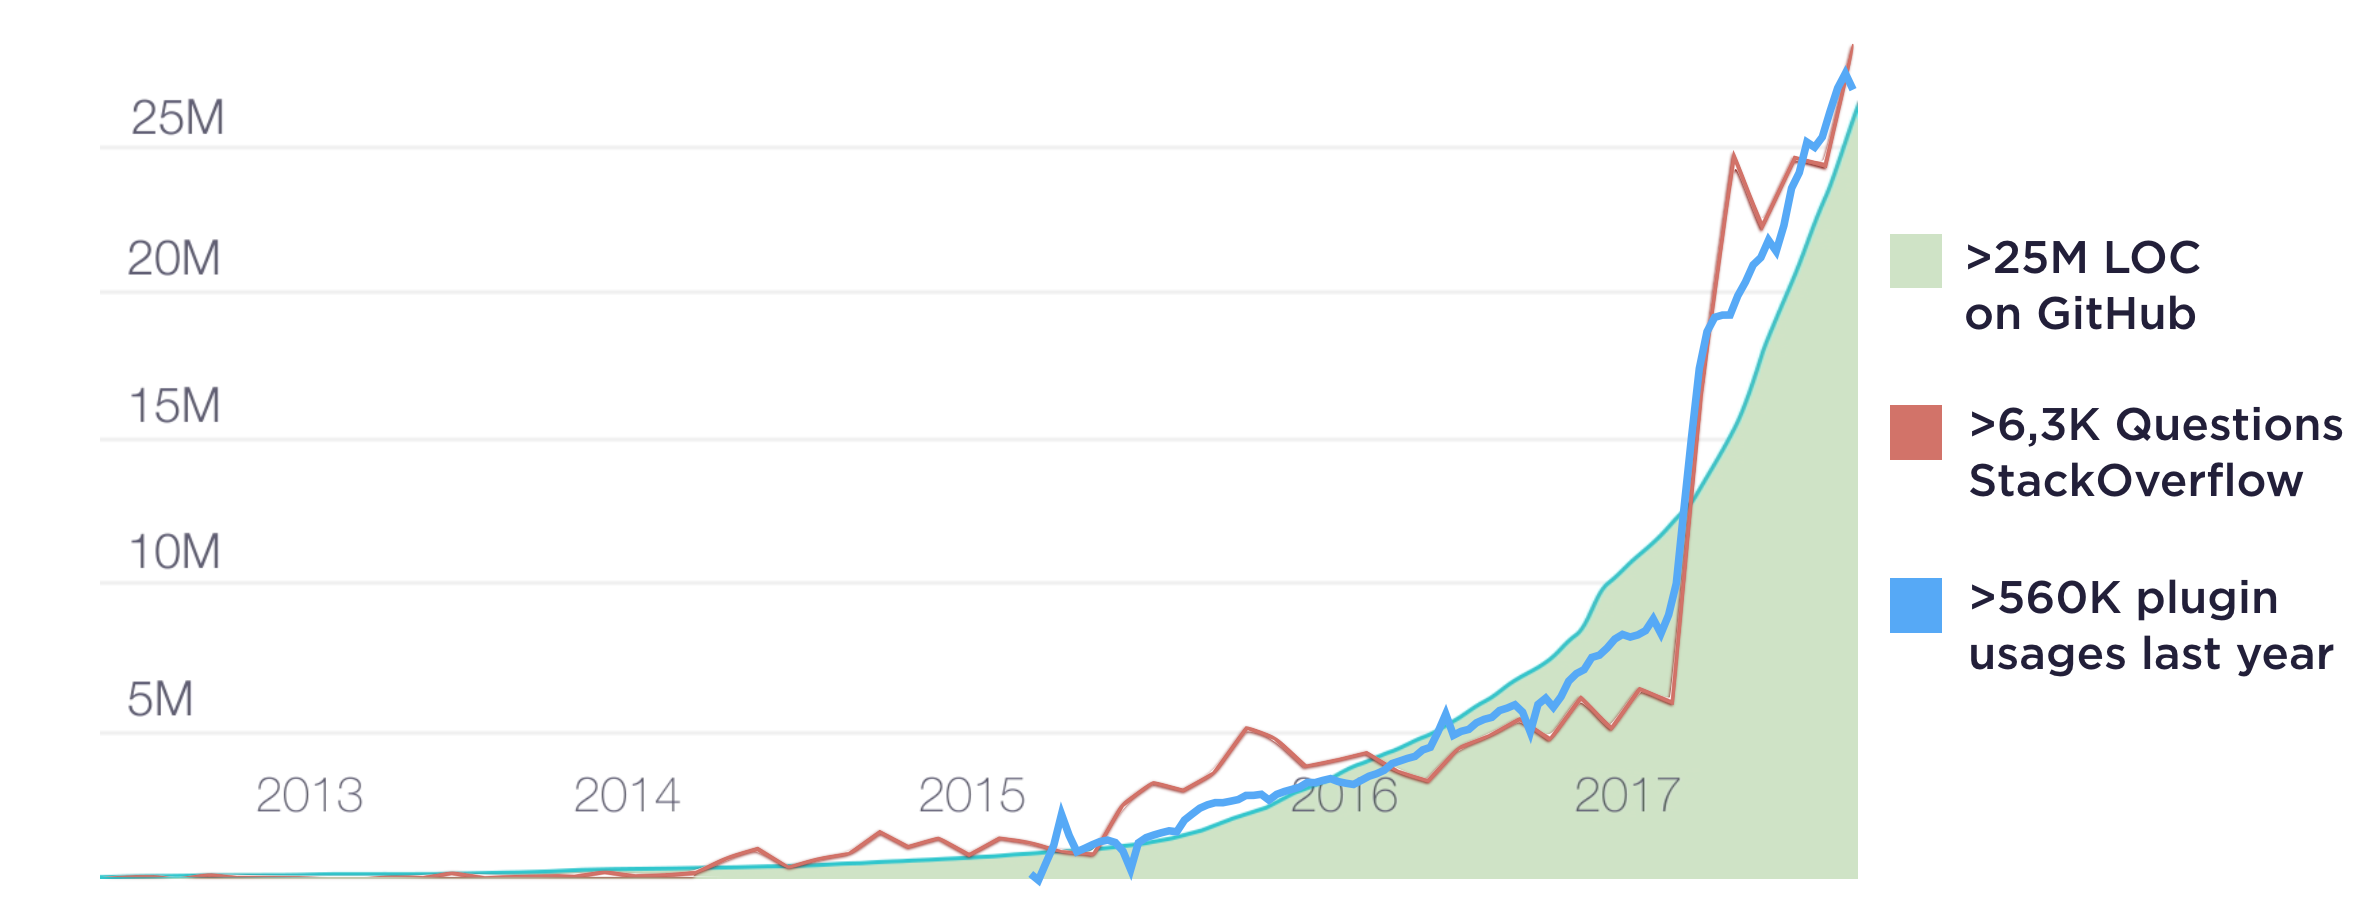
\includegraphics[width=0.95\textwidth]{img/KotlinAdoption.png}
	\caption{Hoeveelheid Kotlin code op GitHub (\cite{JetBrains12})}
	\label{fig:kotlingithub}
\end{figure}

\begin{figure} [ht]
	\centering
	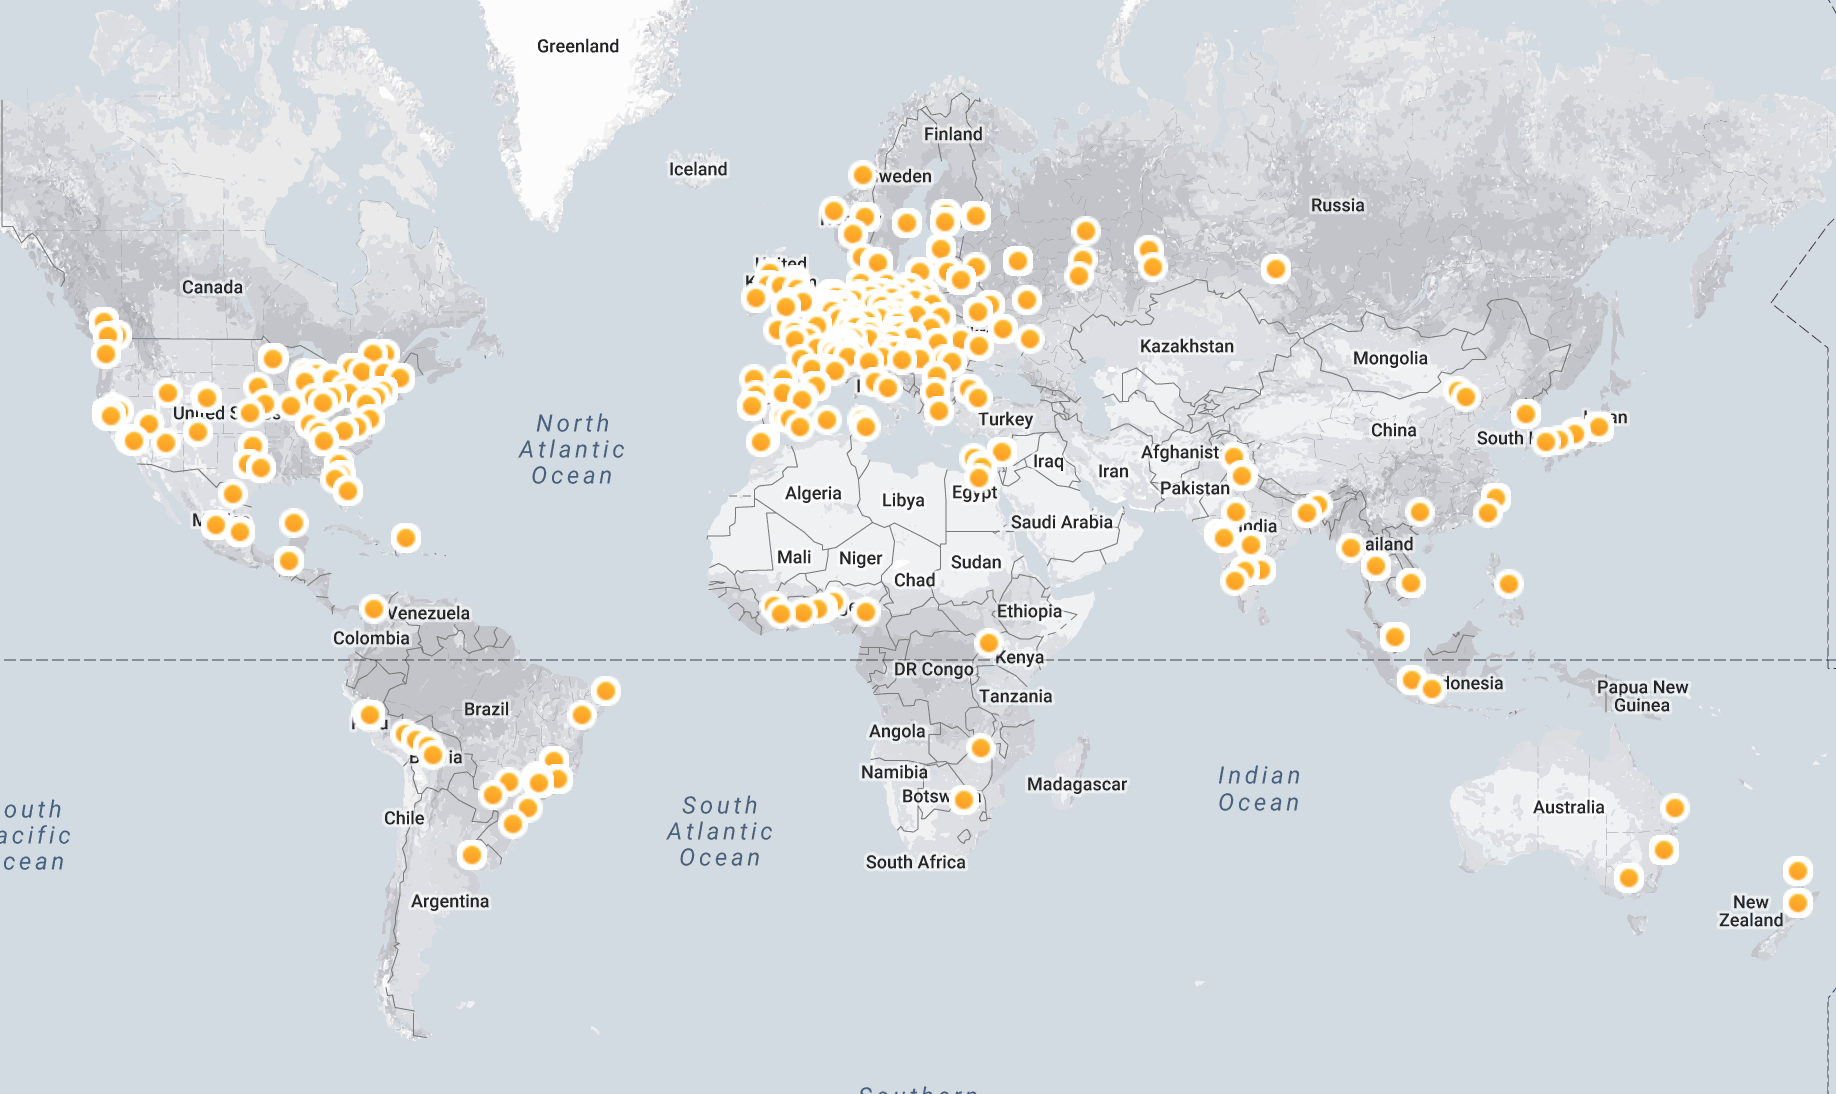
\includegraphics[width=0.95\textwidth]{img/KUGmap.png}
	\caption{Kotlin user groups in de wereld (\cite{JetBrains12})}
	\label{fig:usergroups}
\end{figure}

Volgens statistieken van een Android-software ontwikkelingsbedrijf genaamd AppBrain \autocite{AppBrain}, is Kotlin het beste framework voor Android-applicaties te ontwikkelen. Verschillende veel gebruikte applicaties zoals Netflix, Twitter en Candy Crash bevatten grote delen Kotlin code.

Figuur \ref{fig:usergroups} toont de verschillende user groups over de volledige wereld. Het toont de sterke opkomst van Kotlin over de wereld, met een sterke concentratie in Europa.

\section{Waarom Kotlin?}
\label{sec:whykotlin}
Maar waarom heeft JetBrains besloten om te beginnen met een nieuwe programmeertaal en deze dan later verder uit te bouwen met een cross-platform framework?

Een verklaring die op het internet te lezen is (\cite{TechYourChance}), is dat JetBrains Kotlin heeft uitgevonden om hun eigen productiviteit te vergroten. Ze vonden dat Java niet al hun verwachtingen kon inlossen en daarom moest er een nieuwe programmeertaal op de markt komen. Momenteel hebben ze reeds een groot aantal IDE's ontwikkeld die geschreven zijn in Java. Dat is dan ook de reden dat men een programmeertaal ontwikkeld heeft die naar Java compileerbaar is. Een andere reden zou zijn dat men ontwikkelaars zou willen migreren naar een binnenshuis programmeertaal die gemakkelijker te ondersteunen is.

Anderzijds het feit dat ze kiezen voor een taal die draait op de JVM, betekent dus dat JetBrains niet alle bestaande libraries wil herschrijven, maar hergebruiken. Dit is ook te zien aan de compatibiliteit van beide programmeertalen. Beiden talen zijn volledig compatibel met elkaar. Sectie \ref{sec:Automigration} is hiervan een mooi voorbeeld.

Op 2 augustus 2011 heeft JetBrains, in het jaar dat Kotlin bekend gemaakt werd, een artikel geschreven op hun blog \textcite{JetBrainsNeedKotlin} waarin Dmitry Jemerov, de Kotlin tools team lead, verklaart waarom JetBrains Kotlin heeft ontworpen. In deze blogpost vindt men volgend zin terug: "We willen productiever worden door over te schakelen op een meer expressieve taal.". Ze geven dus duidelijk aan dat men productiever wil worden, maar wil men hiermee bevestigen dat Java enkele tekortkomingen heeft?

%Dit hoofdstuk bevat je literatuurstudie. De inhoud gaat verder op de inleiding, maar zal het onderwerp van de bachelorproef *diepgaand* uitspitten. De bedoeling is dat de lezer na lezing van dit hoofdstuk helemaal op de hoogte is van de huidige stand van zaken (state-of-the-art) in het onderzoeksdomein. Iemand die niet vertrouwd is met het onderwerp, weet er nu voldoende om de rest van het verhaal te kunnen volgen, zonder dat die er nog andere informatie moet over opzoeken \autocite{Pollefliet2011}.

%Je verwijst bij elke bewering die je doet, vakterm die je introduceert, enz. naar je bronnen. In \LaTeX{} kan dat met het commando \texttt{$\backslash${textcite\{\}}} of \texttt{$\backslash${autocite\{\}}}. Als argument van het commando geef je de ``sleutel'' van een ``record'' in een bibliografische databank in het Bib\TeX{}-formaat (een tekstbestand). Als je expliciet naar de auteur verwijst in de zin, gebruik je \texttt{$\backslash${}textcite\{\}}.
%Soms wil je de auteur niet expliciet vernoemen, dan gebruik je \texttt{$\backslash${}autocite\{\}}. In de volgende paragraaf een voorbeeld van elk.

%\textcite{Knuth1998} schreef een van de standaardwerken over sorteer- en zoekalgoritmen. Experten zijn het erover eens dat cloud computing een interessante opportuniteit vormen, zowel voor gebruikers als voor dienstverleners op vlak van informatietechnologie~\autocite{Creeger2009}.

%\lipsum[7-20]
